\section{To take away}
\begin{frame}
	\begin{columns}
		{\scriptsize
		\begin{column}{0.5\textwidth}
			\begin{block}{Simulations}
					\textbf{Jet/SN interaction}
				\begin{itemize}
					\item A post-disruption expansion of the bow-shock, who covers the whole jet
					\item Provokes a jet speed local deceleration of $40\%$
					\item Results in a mass-load of $10^{-4}\,M_{\odot}\,{\rm yr}^{-1}$
					      over the interaction time scale 
					\item Strong mixing with the jet flow after the disruption
				\end{itemize}

		\textbf{Ongoing work} 
			\begin{itemize}
				\item SN exploding close to the jet walls, triggering mixing with the ISM
				\item Add $\vec{B}$ to the simulations with \texttt{Lostrego} (L\'opez-Miralles 2022)
			\end{itemize}
			\end{block}


		\end{column}
			\hspace{-.5cm}
		\begin{column}{0.6\textwidth}
			\begin{exampleblock}{Radiative outcomes}
				\begin{itemize}
					\item Computation of the high energy 
							non-thermal emissions using simplified models\\ (Khangulyan 2014, Bosch-Ramon 2018)
					\item Estimate the possibilities of detection of the 
							current and future detectors (CTAO, Chandra, VLA, etc..) for nearby sources
				\end{itemize}
			\end{exampleblock}

			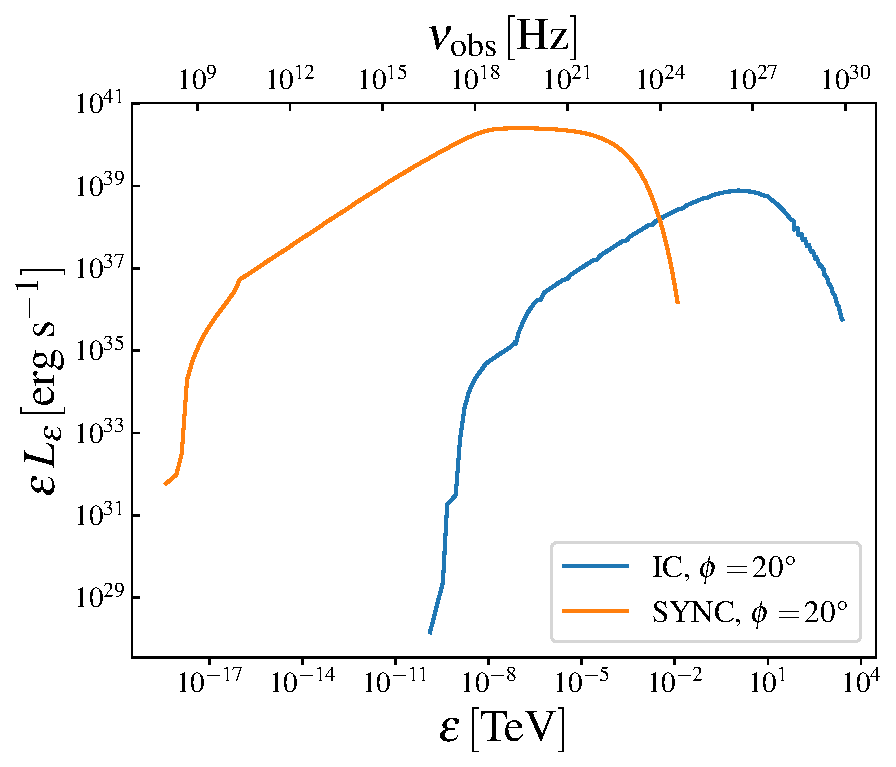
\includegraphics[width=.8\linewidth]{images/eled_ic_sync_hr.pdf}
			\centering
				{\scriptsize Preliminary work on the simulations results}

		\end{column}}
	\end{columns}
\end{frame}

%\section{Backup}

\begin{frame}{Non-thermal emission:\\
	Simplified approach to compute the radiative output}
	\begin{columns}
		{\scriptsize
		\begin{column}{.5\textwidth}
			\begin{block}{Power emitted}
				\begin{itemize}
					\item Non-thermal energy $E_{\rm NT} = \eta U_{\rm cell}$ where $\eta<1$
					\item Broken power-law for the e$^{-}$ distribution with a break 
							energy given by the adiabatic time  \\
					\item \textcolor{blue}{Inverse Compton scattering} + \textcolor{red}{Synchrotron}
%					\quad\quad\quad $N\propto\left\{
%							\begin{array}{ll}
%								E^{-p} & E<E_b\\
%								E^{-(p+1)} & E>E_b
%							\end{array}
%							\right.$

				\end{itemize}
			\end{block}
			\begin{block}{Inverse Compton scattering}
			    \begin{itemize}
				    \item Target photons:\\
						$\rightarrow$ Anisotropic CMB + IR galactic background
					\item Approximate formula for the Thompson+Klein-Nishina regime
						(Khangulyan 2014, Bosch-Ramon 2018)
				\end{itemize}
			\end{block}
		\end{column}
		\begin{column}{.5\textwidth}
			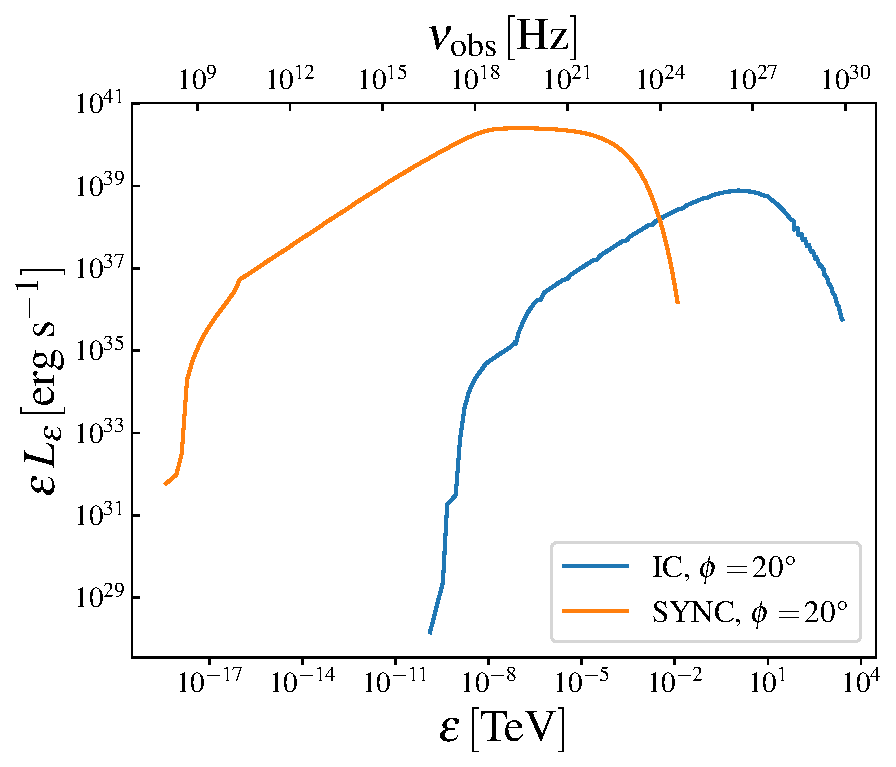
\includegraphics[width=\linewidth]{images/eled_ic_sync_hr.pdf}
			\begin{exampleblock}{SEDs}
				\begin{itemize}
					\item With the given e$^{-}$ distribution, we reach the PeV in IC
					\item The \textcolor{red}{Synchrotron} emission reaches $10^{40}\,{\rm erg}\,{\rm s}^{-1}$
							and the \textcolor{blue}{IC}  $10^{38}\,{\rm erg}\,{\rm s}^{-1}$
				\end{itemize}
			\end{exampleblock}
			\centering
		\end{column}
		}
	\end{columns}
\end{frame}
\begin{frame}{Flux on the line of sight for a source at $z=0.01$ and $\phi=20$°}
	\begin{columns}
		\begin{column}{0.1\textwidth}
				{\small {\bf IC} \\$10^{26}\,{\rm Hz}$  }
		\end{column}
		\begin{column}{\textwidth}
	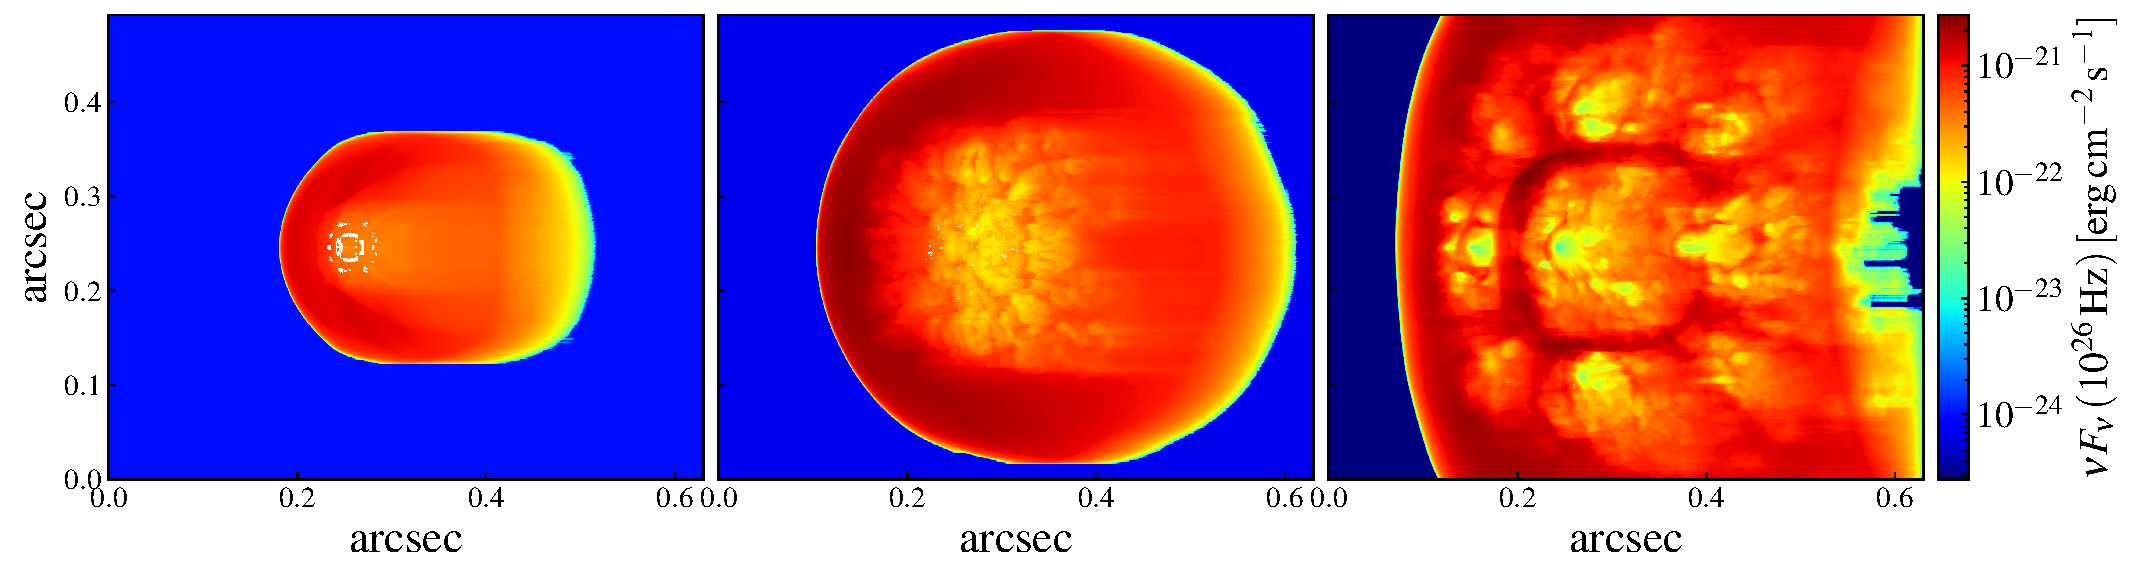
\includegraphics[width=\linewidth]{images/inte_flux_26_ic_5_10_15.pdf}
		\end{column}
	\end{columns}
	\begin{columns}
		\begin{column}{0.1\textwidth}
				{\small{\bf Sync} \\ $10^{20}\,{\rm Hz}$}
		\end{column}
		\begin{column}{\textwidth}
            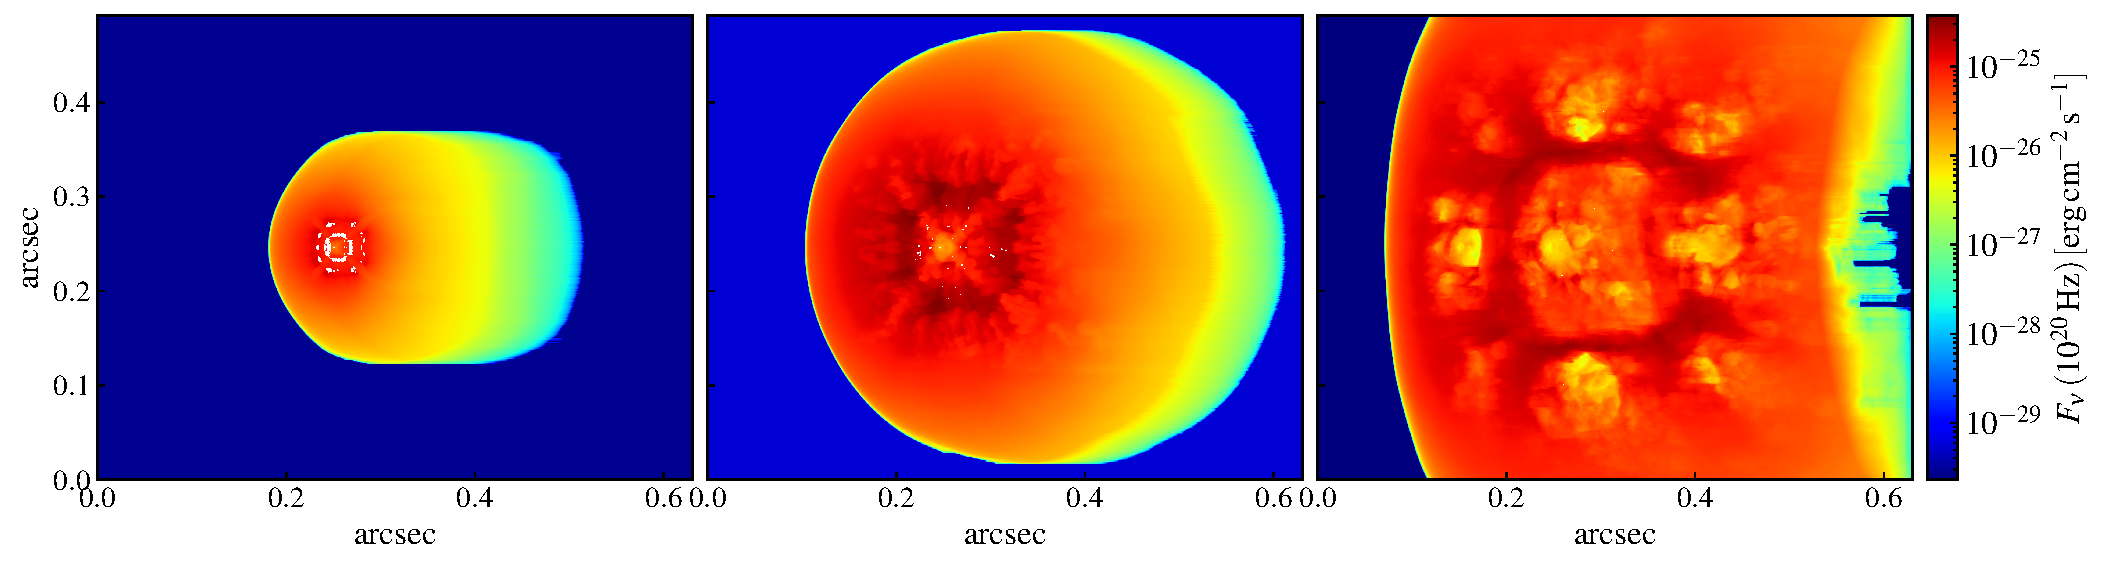
\includegraphics[width=\linewidth]{images/inte_flux_20_sync_5_10_15.pdf}
		\end{column}
	\end{columns}
	\vspace{8pt}
		\hspace{70pt} $1\,{\rm kyr}$ \hspace{60pt} $2\,{\rm kyr}$ \hspace{60pt} $2.9\,{\rm kyr}$
\end{frame}

